\section{Introduction}
\label{section:intro}

\emph{Peer-to-peer} (\p) networks are self-organizing, distributed systems where
participating nodes, called \emph{peers}, act as both resource providers and
resource consumers, in contrast to the traditional \emph{client-server} model
where nodes undertake specific roles.
For over a decade, \p\ networks have been widely deployed and have
enjoyed immense popularity from Internet communities, primarily because
of the great number of features they offer to distributed applications 
built atop them. 
Such diverse features include:  high availability and robustness,
load-balancing, quality of service, scalability, decentralized administration,
and anonymity. 

The peer-to-peer paradigm gave impetus to two ``killer'' applications:
file-sharing and Internet telephony.
The {\sl Napster} file-sharing was widely acknowledged as the 
``fastest growing Internet application ever'' in $2001$ when
$26$ million users shared $80$ million songs.
% File-sharing, originally introduced by
% {\sl Napster} (Section~\ref{section:background}), was widely
% acknowledged by $2001$ as the ``fastest growing Internet application ever" 
% with $26$ million users sharing $80$ million songs.
% % at the height of its popularity. 
Other file-sharing applications followed suit, 
including {\sl Gnutella} and {\sl Limewire} enjoying $3$ 
million concurrently-connected peers as well as 
{\sl BitTorrent} connecting over $150$ million users by the end of $2006$.
\p\ telephony saw explosive growth with the advent of {\sl Skype}.
Since its introduction in $2003$,
{\sl Skype} has become extremely popular with more than $650$ million users 
in $2011$~\cite{skypetotalusers}; on March $5$th, $2012$,  
the astonishing figure of $35$ million concurrently-online users  
was reported~\cite{skypesymusers}.
%%
In addition, a startling number of diverse and successful
applications have been built based on a \p\ architecture. 
Some of them include:
distributed search engines~\cite{yaci}, 
distributed data-storage systems~\cite{kbc_oceanstore_2000,bdet_fsdfs_2000,dkkms_cfs_2001,dr_pastutility_2001,abc_farsite_2002,mmfc_ivy_2002,arla,agebh_dks_2003},
Web caches, archives and publishing systems~\cite{ird_squirrel_2002,bags_youserv_2002,wrc_publius_2000,wm_tangler_2001},
messaging and dissemination applications~\cite{threedegrees,icpp08-pd}, 
event-notification infrastructures~\cite{rkcd_scribe_2001,cdkr_scribe_2002,agebh_dks_2003}, 
naming services~\cite{cmm_chorddns_2002}, 
censor-resistant stores~\cite{cswh_freenet_2001} and
lately, even cloud-based platforms~\cite{mgpj_cloudsnap_2011}.

\p\ systems are implemented using \emph{overlay networks}. 
An overlay network, is a virtual system of nodes and logical links
created above an existing network; overlays provide
added value to the underlying layer by, for instance, offering QoS
content-distribution over the best effort Internet. 
Overlay nodes communicate through \emph{virtual connections} each 
of which may correspond to a path of possibly many physical links 
in the underlying network.
Figure~\ref{figure:overlay} illustrates a simple four-node overlay constructed
over a wide-area network.
%%
\begin{figure}[ht]
\centering
  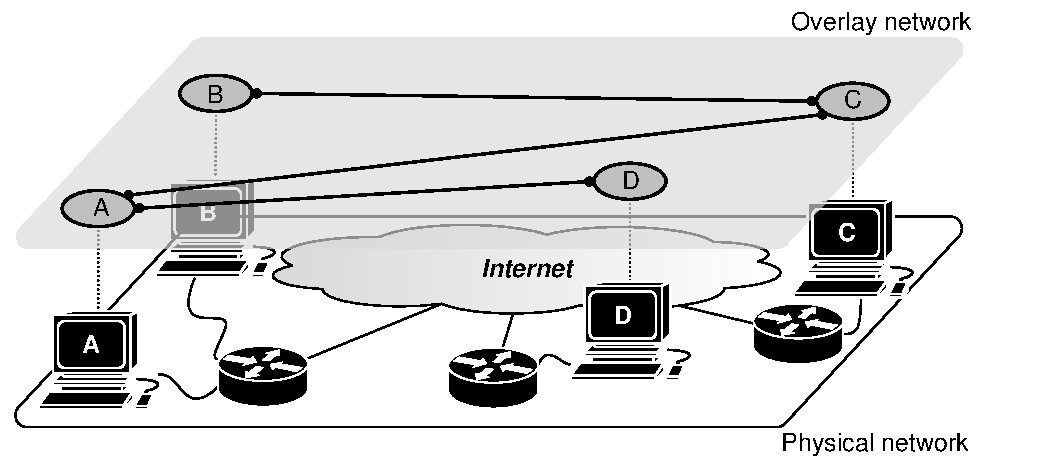
\includegraphics[scale=0.6]{img/pdf/under-over-lay.pdf}
\caption{An example overlay network.}
\label{figure:overlay}
\end{figure}

The single key issue that determines the efficiency of an overlay network,
is how well the overlay maps to the underlying network topology on which it
``rests''. 
Consider two nodes\footnote{In \p\ networks,
the participating nodes are typically user-PCs operating at the edge of the
Internet.} that are connected with each other via a path of overlay links.
If the application running on the nodes, generates heavy traffic along
the overlay path, it would be beneficial to
construct the overlay topology in a way that the number of 
underlying IP links between these two nodes is minimized.
% If the traffic patterns of the application
% are such that traffic flows heavily over the overlay link 
% between the two nodes,
% then it is beneficial to construct the overlay 
% topology such that the number of
% underlying IP links between these two nodes is minimized.
%%
Should the overlay network be constructed so that
it does not match the underlying topology well, 
the inherent \emph{topology mismatch} gives two
significant problems: first, the performance of the application per se, can be
adversely affected since traffic must flow over a larger,
redundant, number of physical hops resulting in poor user experience 
entailing noticeable latencies or jittering. 
%%
Second, other applications running
on the underlying network infrastructure are also adversely affected.
Studies have shown that highly popular \p\ applications contribute 
the largest portion of the overall 
Internet traffic~\cite{seroiu_analysiscds_2002,sen_analyzep2ptraffic_2004,krp_ispfear_2005}, with some reporting that more than $60$\% of this traffic 
to be \p-related~\cite{cachelogic,ipoque2007,ipoque2009};
it was also projected that this traffic would reach
$8\;$\emph{Petabytes}-per-month by the end of $2012$~\cite{multinteligence}. 
Evidently, this constitutes a major burden for 
Internet Service Providers (ISPs) who must route 
all of this traffic to destinations at the edge of the Internet. 
If the \p\ overlay topology is poorly designed, 
the demand on the Internet's backbone infrastructure may 
substantially increase as traffic might have to flow
``back and forth'' several times between two neighboring ISPs
while trying to travel from the source to its destination node
in the overlay.
Hence, it is very critical that \p\ networks be laid out 
in ways that their topology matches, as closely as possible, the 
underlying IP topology.

For over a decade, researchers have extensively investigated  
various aspects of the topology mismatch problem.
The main objective of this paper is to offer a comprehensive 
survey of the work done in this and provide a
taxonomy of the proposed solutions. We point out synergies, as well as
similarities and differences in the published approaches. 
Ultimately, our goal is to help readers sift through 
the voluminous literature, to help them
understand the advantages and disadvantages of each work, and 
to provide them with enough perspective so that 
when the need arises, they are able to
select, amongst the different approaches, the one that is most suitable for
their particular application.
%%
The rest of the paper is organized as follows: 
Section~\ref{section:background} provides background on
overlay architectures including centralized, decentralized
unstructured and decentralized-structured \p\ systems. 
We also formally define the problem of topology mismatch 
% between an overlay and its underlying
% physical network 
and offer the rationale behind our 
evaluation of the techniques discussed in this paper. 
Sections~\ref{section:unstructured} and~\ref{section:structured}
respectively outline the surveyed research efforts 
for decentralized-unstructured and decentralized-structured \p\ systems.
Conclusions can be found in Section~\ref{section:conclusion}.
